\documentclass[10pt]{article}
\usepackage[utf8]{inputenc}
\usepackage[T1]{fontenc}
\usepackage{graphicx}
\usepackage[export]{adjustbox}
\graphicspath{ {./images/} }
\usepackage{amsmath}
\usepackage{amsfonts}
\usepackage{amssymb}
\usepackage[version=4]{mhchem}
\usepackage{stmaryrd}

\title{CHAPTER }

\author{}
\date{}


\newcommand\longdiv[1]{\overline{\smash{)}#1}}

\begin{document}
\maketitle
\begin{center}
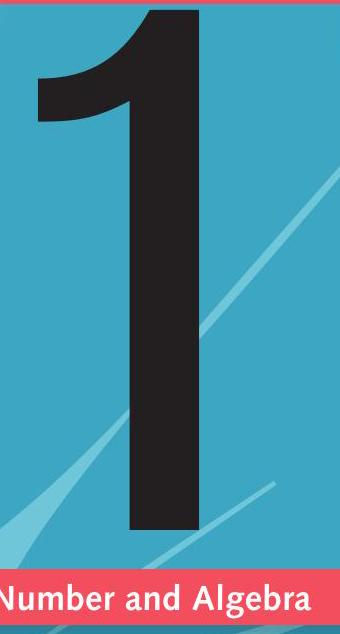
\includegraphics[max width=\textwidth]{2024_05_02_e8cf8b2d35d1e6495e29g-01}
\end{center}

\section*{Whole numbers}
The numbers \(0,1,2,3,4,5,6,7,8,9,10,11, \ldots\) are called the whole numbers. Whole numbers are used for counting objects, such as the number of the people in a room.

Zero ( 0 ) is the first of these numbers. Zero is important because it is used to describe some common situations:

\begin{itemize}
  \item The room is empty. (There are 0 people in the room.)
  \item There are no frogs in my bathroom. (There are 0 frogs in my bathroom.)
\end{itemize}

There is no last whole number, as every whole number is followed by another whole number. The next whole number is obtained by adding 1 to the previous whole number. The list of whole numbers is infinite - it never ends.

The whole numbers are also known as the counting numbers. We use them every day to talk about ideas and describe events and achievements.

The following are some world records from Guinness World Records. Each one is expressed in terms of a whole number.

\begin{itemize}
  \item The greatest number of step-ups completed in 1 hour is 4135.
  \item The greatest number of dominoes stacked end-to-end vertically is 726.
  \item The greatest number of drum beats in 1 minute is 1080.
  \item The greatest number of pancakes tossed in 2 minutes is 416.
  \item The highest first-class cricket score ever is 501, scored by Brian Lara.
\end{itemize}

The operations of addition, subtraction, multiplication and division help to answer further questions about such numbers. For example:

\begin{itemize}
  \item Estimate the record for the greatest number of drum beats in a second. This is found by dividing the number of drum beats in a minute by 60 .
  \item How many pancakes could be tossed in 6 minutes if the record-holder could keep going at the same rate? This is found by multiplying 416 by 3 .
\end{itemize}

Many of the calculations in this chapter should be carried out mentally. Mental calculations will help you build your mathematical skills.

\section*{Whole numbers}
\begin{itemize}
  \item The whole numbers (or counting numbers) are the numbers \(0,1,2,3,4,5,6,7,8,9,10,11, \ldots\)
  \item Zero is the first whole number.
  \item There is no last whole number - the list of whole numbers is infinite.
  \item Counting any collection of objects gives the same answer, whatever order they are counted in.
\end{itemize}

\section*{1 A the number line}
The whole numbers can be represented by points on a line.

Label a point 0 and then mark off equal intervals of any chosen length, always moving to the right. Label the points \(0,1,2,3,4, \ldots\) as shown. The arrow shows that the line continues in the same direction forever. This line is called the number line.

\begin{center}
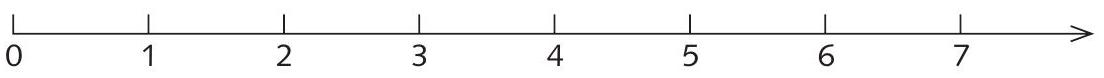
\includegraphics[max width=\textwidth]{2024_05_02_e8cf8b2d35d1e6495e29g-02}
\end{center}

\section*{Less than and greater than}
Any two numbers can be compared with each other. For example, if I have \(\$ 2\) and you have \(\$ 6\), then I have less than you and you have more than me.

On the number line, 2 is to the left of 6 . This is written as \(2<6\). It is read as ' 2 is less than 6 '.

The sharp end of the new symbol < points to the smaller number, 2 , and the open end faces the larger number, 6 .

We can also say that 6 is greater than 2 . This means that 6 is to the right of 2 on the number line. This is written as \(6>2\) and is read as ' 6 is greater than 2 '.

\section*{Less than and greater than}
\begin{itemize}
  \item A whole number, \(a\), is less than another whole number, \(b\), if \(a\) lies to the left of \(b\) on the number line. The symbol \(<\) is used for less than. For example, \(2<6\).
  \item We can also say that a whole number, \(b\), is greater than another whole number, \(a\), if \(b\) lies to the right of \(a\) on the number line. The symbol \(>\) is used for greater than. For example, \(11>4\).
\end{itemize}

\begin{center}
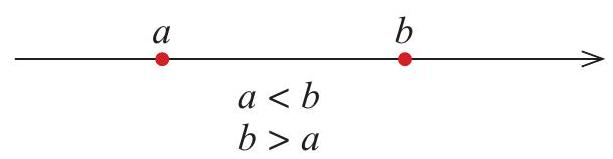
\includegraphics[max width=\textwidth]{2024_05_02_e8cf8b2d35d1e6495e29g-03(1)}
\end{center}

\begin{itemize}
  \item Zero is less than every other whole number.
\end{itemize}

\section*{Example 1}
a List all the whole numbers less than 5.

b List all the whole numbers less than 10 and greater than 1.

\section*{Solution}
a \(0,1,2,3,4\)

b \(2,3,4,5,6,7,8,9\)

\section*{Example 2}
a Draw a number line and on it mark with dots all the whole numbers less than 5 .

b Draw a number line and on it mark all the whole numbers greater than 45 and less than 52.

\section*{Solution}
a\\
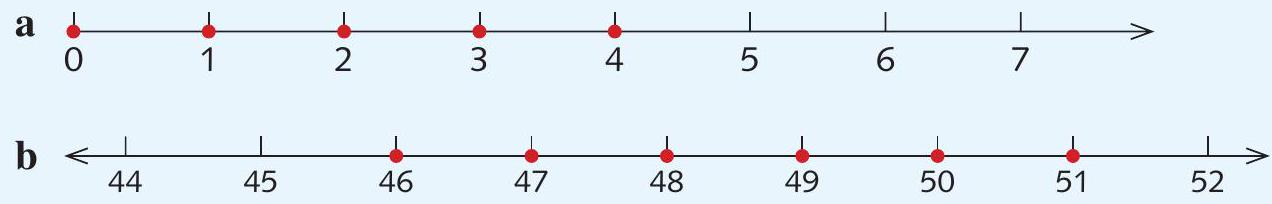
\includegraphics[max width=\textwidth, center]{2024_05_02_e8cf8b2d35d1e6495e29g-03}

\section*{Exercise \(1 \mathrm{~A}\)}
1 a List the whole numbers less than 11.

b List the whole numbers greater than 52 and less than 61 .

2 For each of the following, draw a number line from 0 to 10.

a Mark the numbers \(2,4,6\) and 8 on it.

b Mark the numbers \(1,3,5\) and 7 on it.

c Mark the whole numbers less than 5 on it.

d Mark the whole numbers less than 8 and greater than 2 on it.

3 The manager of an underground railway system decides to save time in the mornings by having one particular train only stop at every third station between stations 1 and 19. The stations are all \(1 \mathrm{~km}\) apart. Show the stations on a number line and mark with a dot each station where the train stops.

\section*{Addition}
Addition is an operation that is carried out on two numbers. You have learned about addition in earlier years, but we will talk about it here to be complete.

The sum is the result of the addition of two numbers.

The sum of two whole numbers, for example, \(6+4\) can be obtained by starting at the number 6 and counting 4 more numbers to the right, as shown on the number line below.

\begin{center}
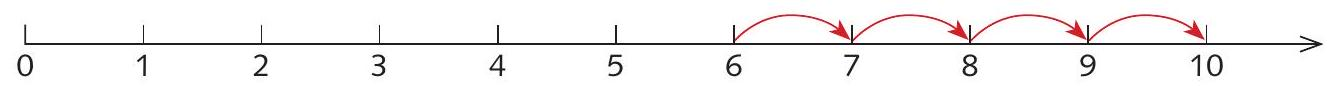
\includegraphics[max width=\textwidth]{2024_05_02_e8cf8b2d35d1e6495e29g-04(1)}
\end{center}

\section*{Making mental addition simpler}
The order in which we perform addition does not matter. For example, \(6+4=4+6\). This can be shown on the number line.

\begin{center}
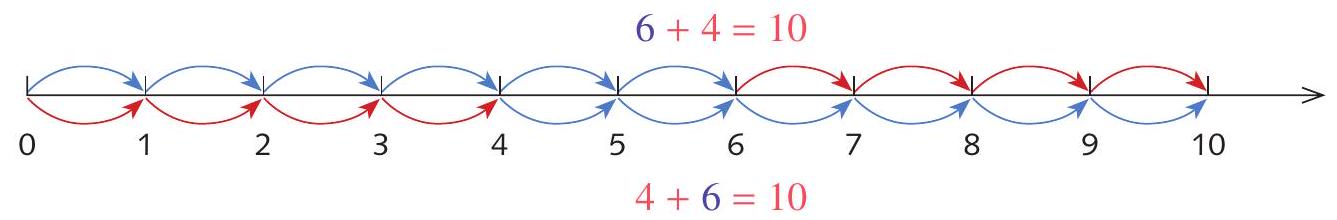
\includegraphics[max width=\textwidth]{2024_05_02_e8cf8b2d35d1e6495e29g-04}
\end{center}

This property is called the commutative law for addition.

The word commutative is related to the word commute. Both words come from the Latin word commutare, which means 'to interchange'.

In mathematics, it is a rule that operations contained in brackets are performed first. When three or more numbers are added together two at a time, it does not matter which two are added together first.

This property is called the associative law for addition. For example:

\[
(2+4)+5=2+(4+5)
\]

When the commutative law and the associative law are used together for addition, the result can be described as the 'any-order property for addition'.

\section*{Any-order property for addition}
A list of whole numbers can be added two at a time in any order to give the same result.

\section*{Using mental addition}
The any-order property for addition is a great help in simplifying arithmetic calculations. Many of them can be done in your head, or mentally.

\section*{Example 3}
Calculate each of the following using the any-order property for addition. (They are set out so that you can see the strategy.)\\
a \(23+41+7+9\)\\
b \(27+55+445+23+7\)

\section*{Solution}
a \(23+41+7+9=(23+7)+(41+9)\)

\[
\begin{aligned}
& =30+50 \\
& =80
\end{aligned}
\]

b \(27+55+445+23+7=(27+23)+(55+445)+7\)

\[
\begin{aligned}
& =50+500+7 \\
& =557
\end{aligned}
\]

\section*{Exercise \(1 B\)}
1 Carry out these additions mentally.\\
a \(15+5\)\\
b \(8+22\)\\
c \(13+7\)\\
d \(74+6\)\\
e \(7+58\)\\
f \(6+38\)\\
g \(8+89\)\\
h \(32+9\)\\
i \(35+27\)\\
j \(42+19\)\\
k \(29+36\)\\
l \(57+86\)

2 Carry out these additions.\\
a \(1+9+33\)\\
b \(2+38+5\)\\
c \(27+6+3\)\\
d \(16+24+5\)\\
e \(61+9+24\)\\
f \(4+42+38\)\\
g \(16+55+27\)\\
h \(72+19+26\)

3 Do these computations using the techniques introduced so far.\\
a \(22+17+18+23\)\\
b \(14+18+76+92\)\\
c \(13+27+64+6\)\\
d \(25+32+15+18\)\\
e \(15+34+26+35\)\\
f \(12+19+18+1\)

4 Carry out these additions.\\
a \(243+57\)\\
b \(567+43\)\\
c \(328+22\)\\
d \(786+24\)\\
e \(435+25\)\\
f \(963+57\)\\
g \(486+524\)\\
h \(364+251\)

5 Three cows produced 29 litres, 47 litres and 23 litres of milk in one day.

How much milk did they produce in total?

6 A tiler laid 267 tiles in the kitchen, 20 tiles in the laundry and 113 tiles in the bathroom. How many tiles did he lay in total?

7 On the first day of my holidays, I travelled 85 kilometres from my home in Victor Harbor to Adelaide, then 516 kilometres from Adelaide to Broken Hill. The next day I travelled 298 kilometres from Broken Hill to Mildura.

How many kilometres did I travel in the first two days of my trip?

8 A busker collected \(\$ 8.00, \$ 13.00, \$ 4.00\) and \(\$ 12.00\) over four days. How much did she earn?

9 In three Year 7 classes, 27 students, 31 students and 26 students attended roll call one morning. How many Year 7 students were present?

10 I picked 18 daffodils from my garden on Monday, 3 on Tuesday, 27 on Wednesday, 6 on Thursday and 12 on Friday. How many daffodils did I pick over the five days?

11 In one week, Sam read four books. The first book had 312 pages, the second 175, the third 48 and the fourth 98 . How many pages did Sam read in the week?

12 a By appropriately pairing numbers, carry out the addition \(1+2+3+4+5+6+7+8+9\). b Use the same idea to find the sum of numbers from 1 to 99 inclusive.

\section*{The standard addition algorithm}
An algorithm is a set of procedures or steps for performing a task. In this section we look at an algorithm for addition.

We will use the two-digit numbers 15 and 27 to demonstrate the addition algorithm.

\[
\begin{array}{rrl}
1 & 5 & (1 \text { ten and } 5 \text { ones) } \\
+2 & 7 & (2 \text { tens and } 7 \text { ones) } \\
4 & 2 & \text { (4 tens and } 2 \text { ones) }
\end{array}
\]

This is explained by saying, as we add the ones:

5 ones +7 ones \(=12\) ones

and 12 ones is 1 ten and 2 ones

Write 2 in the ones column and carry 1 ten to the tens column.

As we add the tens, we say:

\[
1 \text { ten }+2 \text { tens }+1 \text { ten }=4 \text { tens }
\]

We then write 4 in the tens column.

The final answer is 42 .

This technique can be extended to three or more numbers with different numbers of digits.

\section*{Example 4}
Complete the following additions.\\
a\\
935\\
\(\begin{array}{llll}23 & 8 & 2 \\ & & \end{array}\)\\
\(+\quad 97\)\\
b\\
\(\begin{array}{llll}7 & 1 & 3 & 6\end{array}\)\\
\(+\underline{8095}\)

\section*{Solution}
\(\mathbf{a}\)\\
\(\begin{array}{llll}9 & 3 & 5\end{array}\)\\
\(\begin{array}{llll}2 & 3 & 8 & 2\end{array}\)\\
\(+\begin{array}{r}1297 \\ \hline 3414 \\ \hline\end{array}\)\\
b

\begin{center}
\begin{tabular}{r}
7136 \\
\(+\quad 8095\) \\
\hline
5231 \\
\hline
\end{tabular}
\end{center}

\section*{Exercise \(1 C\)}
1 Work out the answers to these additions by using the standard algorithm.\\
a \(721+630\)\\
b \(235+549\)\\
c \(109+872\)\\
d \(468+951\)\\
e \(973+296\)\\
f \(2107+989\)\\
g \(1432+3791\)\\
h \(793+274+473\)\\
i \(8693+7392\)\\
j \(9999+32\)

2 Work out the answers to these additions.\\
a \(37+129+1647\)\\
b \(9230+839+61\)\\
c \(829+1083+437\)\\
d \(72+274+391+28\)\\
e \(254+194+482+53\)\\
f \(632+106+7+270\)

3 For each of the following, find the missing digits ( \(\star\) ) to make the addition correct.\\
a

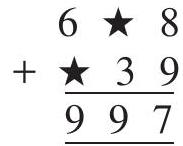
\includegraphics[max width=\textwidth, center]{2024_05_02_e8cf8b2d35d1e6495e29g-07(3)}\\
b \(\quad 8 \star 4\)

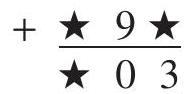
\includegraphics[max width=\textwidth, center]{2024_05_02_e8cf8b2d35d1e6495e29g-07(2)}\\
c \(\begin{array}{r}919 \\ +\begin{array}{r}89 \star \\ \hline 1 \star 18\end{array}\end{array}\)\\
d

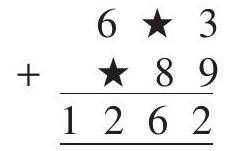
\includegraphics[max width=\textwidth, center]{2024_05_02_e8cf8b2d35d1e6495e29g-07}\\
e

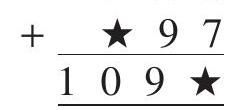
\includegraphics[max width=\textwidth, center]{2024_05_02_e8cf8b2d35d1e6495e29g-07(1)}\\
f \(\quad 3 \star 3\)\\
\(+\begin{array}{r}77 \star \\ \star 110\end{array}\)

4 Make six different three-digit numbers from the digits 4,7 and 8 . What is their sum?

5 Find the sum of:

a three hundred and sixty-seven and six hundred and twenty-seven

b four hundred and twenty-four and five thousand, three hundred and twenty-six

6 The odometer of a car read 54987 kilometres at the beginning of a journey of 765 kilometres. What did it read at the end of the journey?

7 A shop had three employees. The manager received \(\$ 976\) per week and the senior assistant received \(\$ 654\) per week. The junior assistant earned \(\$ 443\) per week. What was the total weekly wages bill for the shop?

8 The Amazon River is 6436 kilometres in length and the Nile River is 234 kilometres longer. What is the length of the Nile?

9 The populations of five ant farms were determined at the end of each of three months.

\begin{center}
\begin{tabular}{|l|c|c|c|c|c|}
\hline
 & Ant farm A & Ant farm B & Ant farm C & Ant farm D & Ant farm E \\
\hline
March & 97 & 597 & 143 & 89 & 13 \\
\hline
April & 113 & 603 & 89 & 432 & 28 \\
\hline
May & 214 & 411 & 17 & 729 & 164 \\
\hline
\end{tabular}
\end{center}

a List the ant farms in order of increasing size of their populations at the end of March.

b What was the population of Ant farm A at the end of May?

c Which of the ant farms had a population greater than 100 at the end of April?

d What was the total population of all five ant farms at the end of May?

10 Complete the following to make the addition correct.

\begin{center}
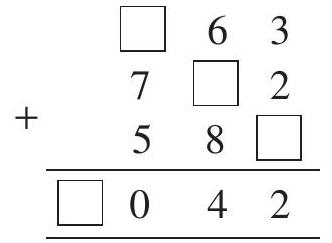
\includegraphics[max width=\textwidth]{2024_05_02_e8cf8b2d35d1e6495e29g-08(2)}
\end{center}

\section*{1 Subtiaction}
A whole number can be subtracted from a larger whole number. The result is called the difference of the two numbers. For example, \(8-5=3\). The difference of 8 and 5 is 3 .

\section*{Subtracting as 'taking away'}
If you have 5 items and you take 2 away, the number remaining is \(5-2=3\).

For example, I had 5 pencils but my sister took 2 away, so now I have 3.

On a number line, this is illustrated by moving two numbers to the left.

\begin{center}
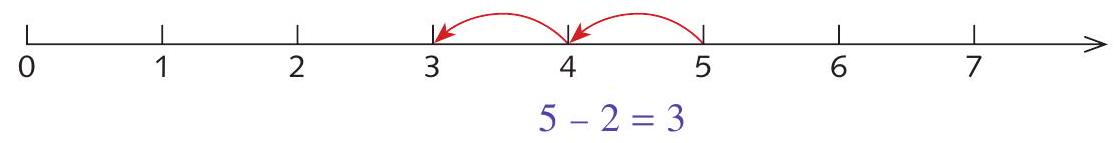
\includegraphics[max width=\textwidth]{2024_05_02_e8cf8b2d35d1e6495e29g-08(1)}
\end{center}

\section*{Subtracting as 'adding on'}
Another way of thinking about the subtraction \(5-2\) is to ask 'What is the difference?' or 'What do you add on to 2 to get to 5?' Subtraction can also be thought of as an alternative way of expressing the addition \(2+3=5\).

\begin{center}
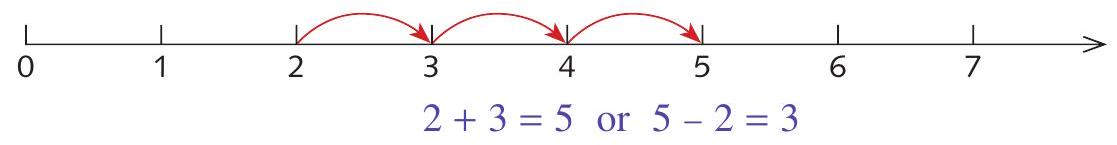
\includegraphics[max width=\textwidth]{2024_05_02_e8cf8b2d35d1e6495e29g-08}
\end{center}

One example of this is 'I have 5 pencils and my brother has 2, so I have 3 more pencils than my brother'.

\section*{Subtraction of whole numbers}
\begin{itemize}
  \item A whole number can always be subtracted from a larger whole number to give the difference of the two numbers.
  \item 'I had 8 but someone took away 5' can be expressed as \(8-5\).
  \item 'I have 8 and she has 5, so I have 3 more' can also be expressed as \(8-5\).
  \item Subtraction is the reverse process of addition. For example, \(8-5=3\) is equivalent to saying \(3+5=8\).
\end{itemize}

\section*{Mental subtraction}
Here are three ways to perform the subtraction \(100-67\).

1 Count on from the smaller number to the larger number.

Going from 67 to 70 requires counting on 3.

Going from 70 to 100 requires counting on 30.

Therefore \(100-67=33\).

2 Subtract the 60 and then the 7.

\[
\begin{aligned}
100-67 & =100-60-7 & & \text { (First subtract the 60.) } \\
& =40-7 & & \text { (Then subtract the 7.) } \\
& =33 & &
\end{aligned}
\]

3 Take away 70 and then add 3.

\[
\begin{aligned}
100-67 & =100-70+3 & & \\
& =30+3 & & \text { (First subtract 70, which is } 3 \text { too many, } \\
& =33 & & \text { so then we add the 3.) }
\end{aligned}
\]

\section*{Example 5}
Carry out these subtractions mentally.\\
a \(39-31\)\\
b \(27-8\)\\
c \(183-96\)

\section*{Solution}
a One way you might choose to do this is to subtract the 30 , then the 1 .

\[
\begin{aligned}
39-31 & =39-30-1 \\
& =9-1 \\
& =8
\end{aligned}
\]

b One way you might choose to do this is to first subtract 7 from 27 , then subtract 1 .

\[
\begin{aligned}
27-8 & =27-7-1 \\
& =20-1 \\
& =19
\end{aligned}
\]

c One way you might choose to do this is to take away 100 , then add 4.

\[
\begin{aligned}
183-96 & =183-100+4 \\
& =83+4 \\
& =87
\end{aligned}
\]

\section*{Zero}
The number zero is very important in arithmetic. When you add 0 to a number or subtract 0 from a number, the result is the original number.

For example, \(2+0=2\) and \(2-0=2\). When a whole number is subtracted from itself, the answer is zero. For example, \(5-5=0\).

\section*{The standard subtraction algorithms}
We can set out subtraction in the familiar column form.

\[
\begin{array}{r}
56 \\
-24 \\
\hline 32 \\
\hline
\end{array}
\]

In the previous example, \(6>4\) and \(5>2\) so the subtraction is very easy. What can we do if this is not the case?

Consider 54-26. We set this out in column form and we work on the units column before the tens column. (In general, we work from right to left across the columns.)

\section*{Method 1: Equal addition}
\(5^{14}\) Since \(6>4\), we add 10 to the 54 by changing the 4 to 14 , which we write as \({ }^{1} 4\).

\(-2_{1} 6\) To restore the correct answer, we add 10 to the 26, making it 36; we do this

\(\sqrt{2} 8\) by writing 3 as \(2_{1}\). We can now subtract in each column to get 28 .

\section*{Method 2: Trading or decomposition}
\({ }^{4} 8{ }^{1} 4\) Think of 54 as 5 tens and 4 ones, and 26 as 2 tens and 6 ones.

\begin{itemize}
  \item 26 Now write 54 as 4 tens and 14 ones, and subtract 2 tens and 6 ones to get
\end{itemize}

\(\overline{28} 2\) tens and 8 ones.

It does not matter which of the two methods you use - it is your choice.

\section*{Example 6}
Carry out the following subtractions.\\
a \(456-278\)\\
b \(20007-7986\)

\section*{Solution}
a Method 1

\begin{center}
\begin{tabular}{r}
\(4{ }^{1} 5 \quad{ }^{1} 6\) \\
\(-2_{1} \quad 7_{1} 8\) \\
\hline
1788 \\
\hline
\end{tabular}
\end{center}

b Method 1

\[
\begin{array}{r}
2{ }^{1} 02^{1} 0{ }^{1} 07 \\
-\quad 179_{1} 86 \\
\hline 12021 \\
\hline 122
\end{array}
\]

a Method 2

\begin{center}
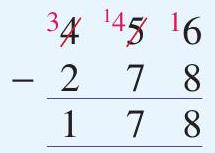
\includegraphics[max width=\textwidth]{2024_05_02_e8cf8b2d35d1e6495e29g-10}
\end{center}

b Method 2

\begin{center}
\begin{tabular}{rrrrr}
1 &  &  &  &  \\
1 & \({ }^{9}\) & \({ }^{9}\) &  & 1 \\
 &  & 7 &  &  \\
 & 7 & 9 & 8 & 6 \\
\hline
1 & 2 & 0 & 2 & 1 \\
\hline
\end{tabular}
\end{center}

\section*{Exercise 1D}
Example 5 Carry out these subtractions mentally.\\
a \(28-22\)\\
b \(273-68\)\\
c \(350-47\)\\
d \(94-66\)\\
e \(137-53\)\\
f \(167-59\)\\
g \(475-95\)\\
h \(1008-17\)

2 Do each of these computations by working from left to right.\\
a \(8+7-7\)\\
b \(8+12-12-8\)\\
c \(19-7+8-19\)\\
d \(56-11+11\)\\
e \(38-18-1+19\)\\
f \(101-11+11\)

3 Carry out these subtractions.\\
a \(562-387\)\\
b \(921-428\)\\
c \(405-286\)\\
d \(813-619\)

4 Carry out these subtractions.\\
a \(3456-234\)\\
b \(18502-7862\)\\
c \(22788-19999\)

5 Copy and then complete each subtraction by finding a digit for each \(\star\).\\
a \(\quad 76\)\\
\(-\underline{2 \star}\)\\
b

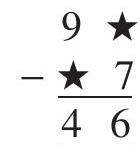
\includegraphics[max width=\textwidth, center]{2024_05_02_e8cf8b2d35d1e6495e29g-11(1)}\\
c \(\begin{array}{r}23 \star \star \\ -\star \star 97 \\ \hline \quad 39 \\ \hline\end{array}\)\\
d\\
\(-\begin{array}{r}4 \star 9 \\ \hline 734\end{array}\)\\
\(\mathbf{e}\)\\
\(\begin{array}{r}\star 76 \star \\ -\quad 43 \\ \hline 1918 \\ \hline\end{array}\)\\
f \(537 \star\)

\begin{center}
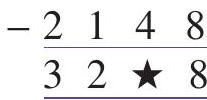
\includegraphics[max width=\textwidth]{2024_05_02_e8cf8b2d35d1e6495e29g-11}
\end{center}

6 Complete each statement by filling in the boxes with numbers that make the statement true.

a \(3+7=10\) is equivalent to \(\square-3=7\)

b \(18+\square=27\) is equivalent to \(\square-18=9\)

c \(42+26=\square\) is equivalent to \(\square-26=42\)

d \(\square+\square=144\) is equivalent to \(144-\square=81\)

7 Bill has \(\$ 456\) more than Anna. Bill has \(\$ 3789\). How much does Anna have?

8 During the last school holidays, Stephen drove from Brisbane to Cairns along the Bruce Highway. He set his trip meter to zero when he left home. It showed \(1236 \mathrm{~km}\) at Townsville and \(1586 \mathrm{~km}\) on his arrival in Cairns. How far did he drive between Townsville and Cairns?

9 Melissa had invited 1534 people to attend a fundraising event, and 204 people indicated they would not be able to attend. How many people did Melissa expect to come to the event?

10 Australia scored 246 and England scored 196 in a one-day cricket match. What was the winning margin? That is, how many more runs did Australia score than England?

11 A town with a population of 34827 has 18439 adults. How many children are there?

1265376 tickets were sold for a concert. The venue had seating for 75000 people. How many more tickets could be sold to fill every seat?

\section*{Multiplication}
Any two numbers can be multiplied together. The result is called the product of the numbers.

The product of 5 and 3 is \(5 \times 3=15\).

This product can be represented by a rectangular array of counters with 3 rows and 5 columns.

(An array of 5 rows of 3 columns will do just as well.)

\begin{center}

\includegraphics[max width=\textwidth]{2024_05_02_e8cf8b2d35d1e6495e29g-12(1)}
\end{center}

Multiplication can also be represented using areas. For example, the rectangle shown has side lengths of \(5 \mathrm{~cm}\) and \(3 \mathrm{~cm}\). Each of the smaller squares shown has side length \(1 \mathrm{~cm}\). The area of the rectangle is \(15 \mathrm{~cm}^{2}\).

\begin{center}
\begin{tabular}{|l|l|l|l|l|}
\hline
 &  &  &  &  \\
\hline
 &  &  &  &  \\
\hline
 &  &  &  &  \\
\hline
\end{tabular}
\end{center}

We have used centimetres here, but any unit of length could be used.

Multiplication by whole numbers can also be illustrated on a number line by using repeated addition. For example:

\begin{center}
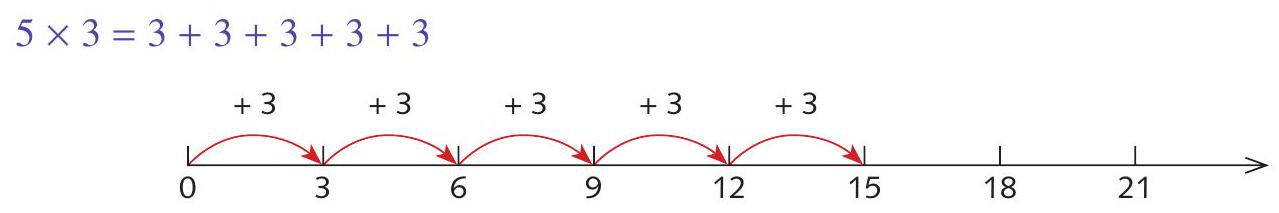
\includegraphics[max width=\textwidth]{2024_05_02_e8cf8b2d35d1e6495e29g-12}
\end{center}

or \(3 \times 5=5+5+5\)

\begin{center}
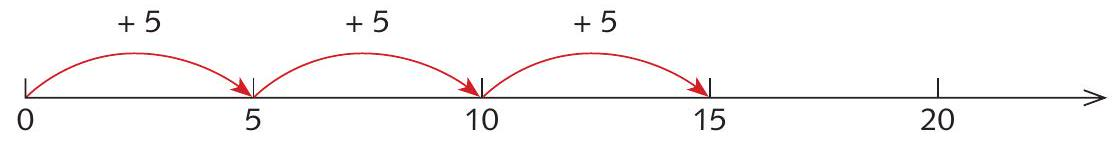
\includegraphics[max width=\textwidth]{2024_05_02_e8cf8b2d35d1e6495e29g-12(2)}
\end{center}

\section*{Zero and one}
When you multiply any number by 0 , the result is 0 . When you multiply any number by 1 , the result is the number you started with. For example:

\[
7 \times 0=0 \quad \text { and } \quad 2 \times 1=2
\]

\section*{Multiplying by \(10,100,1000, \ldots\)}
Multiplying by powers of \(10-\) that is, \(10,10 \times 10=100,10 \times 10 \times 10=1000\) and so on - is straightforward.

\[
\begin{array}{ll}
2 \times 10=20 & 32 \times 10=320 \\
2 \times 100=200 & 32 \times 100=3200 \\
2 \times 1000=2000 & 32 \times 1000=32000 \\
2 \times 10000=20000 & 32 \times 10000=320000
\end{array}
\]

\section*{Example 7}
Perform each multiplication.\\
a \(23 \times 0\)\\
b \(33 \times 1\)\\
c \(43 \times 10\)\\
d \(73 \times 100\)\\
e \(93 \times 1000\)

\section*{Solution}
a \(23 \times 0=0\)\\
b \(33 \times 1=33\)\\
c \(43 \times 10=430\)\\
d \(73 \times 100=7300\)\\
e \(93 \times 1000=93000\)

\section*{Laws for multiplication}
From the diagrams on the previous page, you can see that \(5 \times 3=3 \times 5\). This is an example of the commutative law for multiplication.

Remember that the convention in mathematics is that operations inside brackets are performed first. For three or more numbers multiplied together, two at a time, it does not matter which multiplication you do first. For example:

\[
\begin{array}{rlrl}
(5 \times 3) \times 4 & =15 \times 4 & 5 \times(3 \times 4) & =5 \times 12 \\
& =60 & & =60
\end{array}
\]

That is:

\[
(5 \times 3) \times 4=5 \times(3 \times 4)
\]

This illustrates that the associative law also holds for multiplication. The two rules together show that for strings of multiplications, order does not matter. This result can be described as the 'any-order property for multiplication'.

\section*{Any-order property for multipleation}
Whole numbers can be multiplied two at a time in any order to give the same result.

For example:

\[
\begin{aligned}
4 \times 7 \times 5 & =4 \times 5 \times 7 \\
& =20 \times 7 \\
& =140
\end{aligned}
\]

\section*{Example 8}
Use the any-order property for multiplication to work out the following calculations.\\
a \(5 \times 7 \times 3 \times 2\)\\
b \(20 \times 12 \times 5\)

Solution

a \(5 \times 7 \times 3 \times 2=5 \times 2 \times 7 \times 3\)

\[
\begin{aligned}
& =10 \times 21 \\
& =210
\end{aligned}
\]

\[
\text { b } \begin{aligned}
20 \times 12 \times 5 & =20 \times 5 \times 12 \\
& =100 \times 12 \\
& =1200
\end{aligned}
\]

\section*{Properties of multiplication}
\begin{itemize}
  \item Multiplication of whole numbers can be thought of as repeated addition:
\end{itemize}

\(5 \times 3=3+3+3+3+3\) or \(5 \times 3=5+5+5\)

\begin{itemize}
  \item The commutative law and the associative law hold for multiplication:\\
\(3 \times 4=4 \times 3\)\\
(commutative law)\\
\((5 \times 2) \times 3=5 \times(2 \times 3)\)\\
(associative law)
  \item The any-order property for multiplication says that a list of whole numbers can be multiplied two at a time in any order to give the same result:
\end{itemize}

\[
\begin{aligned}
2 \times 6 \times 100 \times 4 \times 7 \times 25 & =(7 \times 6 \times 2) \times(4 \times 25) \times 100 \\
& =840000
\end{aligned}
\]

\section*{Exercise \(1 E\)}
1 Perform each multiplication.\\
a \(17 \times 10\)\\
b \(89 \times 0\)\\
c \(100 \times 1\)\\
d \(18 \times 1000\)\\
e \(120 \times 100\)\\
f \(100 \times 100\)\\
g \(1000 \times 73\)\\
h \(10000 \times 100\)\\
i \(67430 \times 1000\)

2 Carry out each calculation, using the any-order property for multiplication.\\
a \(25 \times 4 \times 6\)\\
b \(5 \times 26 \times 2\)\\
d \(50 \times 49 \times 2\)\\
c \(5 \times 43 \times 20\)\\
e \(16 \times 5 \times 40\)\\
g \(1 \times 34 \times 20\)\\
f \(13 \times 6 \times 0\)\\
h \(6 \times 10 \times 10 \times 2\)\\
i \(3 \times 7 \times 4 \times 5\)

3 Fill in each box with a number to make the statements true.

a \((3 \times 2) \times 7=3 \times(\square \times 7)\)

b \((5 \times 9) \times(2 \times 8)=9 \times 8 \times(\square \times 2)\)

4 Ian has 13 jars, each containing 20 olives. If he decides to redistribute the olives equally among 20 jars, how many olives will there be in each jar?

5 Six friends buy a large box of jelly snakes. The snakes come in 5 different colours. How many snakes are needed so that every person has two of each colour?

6 Bricks are arranged on a concrete floor in 12 rows of 25, and stacked 4 bricks high. How many bricks are there in total?

7 Holly has prepared 28 bags of lollies for her birthday party. Each bag has 9 lollies in it. She makes these into 14 new bags when some of her friends do not turn up. How many lollies will each person now receive?

\section*{1. combinations of operations and the distributive law}
As soon as there is more than one type of operation in a calculation (for example, both addition and multiplication), we need a set of rules about the order in which the operations are to be performed. These are some of the rules.

\section*{Order of operations}
\begin{itemize}
  \item Work out the calculations inside brackets first.
  \item In the absence of brackets, carry out operations in the following order:
  \item multiplication from left to right, then
  \item addition and subtraction from left to right.
\end{itemize}

This means that:

\[
\begin{aligned}
5 \times 3+2 & =15+2 \\
& =17
\end{aligned}
\]

Brackets can be used to force the addition to be done first. For example:

\[
\begin{aligned}
5 \times(3+2) & =5 \times 5 \\
& =25
\end{aligned}
\]

We will revisit and add to these rules in later sections of this chapter.

\section*{Example 9}
Carry out each of the following calculations.\\
a \(3 \times 7-4\)\\
b \(3 \times(7-4)\)\\
c \(5 \times 6+8\)\\
d \(7 \times(11+4)\)\\
e \(3+4 \times 2\)\\
f \(25-6 \times 3\)

Solution\\
a \(3 \times 7-4=21-4\)\\
\(=17\)\\
b \(\begin{aligned} 3 \times(7-4) & =3 \times 3 \\ & =9\end{aligned}\)\\
c \(5 \times 6+8=30+8\)\\
\(=38\)\\
d \(7 \times(11+4)=7 \times 15\)\\
e \(3+4 \times 2=3+8\)\\
\(=105\)\\
f \(25-6 \times 3=25-18\)\\
\(=11\)\\
\(=7\)

\section*{The distributive law}
When multiplying, it is sometimes useful to express one of the numbers you are multiplying as a sum of two other numbers. For example:

\[
\begin{aligned}
6 \times 105 & =6 \times(100+5) \\
& =6 \times 100+6 \times 5 \\
& =600+30 \\
& =630
\end{aligned}
\]

This is an example of the distributive law for multiplication over addition. Using the distributive law can often help you to do multiplications more easily.

Using the distributive law for multiplication over subtraction can also help to make a multiplication easier. For example:

\[
\begin{aligned}
85 \times 98 & =85 \times(100-2) \\
& =(85 \times 100)-(85 \times 2) \\
& =8500-170 \\
& =8330
\end{aligned}
\]

\section*{Example 10}
Carry out each of the following computations, using the distributive law.

a \(106 \times 8\)

b \(43 \times 7+43 \times 3\)

c \(97 \times 88\)

\section*{Solution}
The following are possible methods.

\[
\begin{aligned}
& \text { a } 106 \times 8=(100+6) \times 8 \\
& =100 \times 8+6 \times 8 \\
& =800+48 \\
& =848
\end{aligned}
\]

b \(7 \times 43+3 \times 43=(7+3) \times 43\)

\[
=430
\]

c \(97 \times 88=88 \times(100-3)\)

\[
\begin{aligned}
& =88 \times 100-88 \times 3 \\
& =8800-264 \\
& =8536
\end{aligned}
\]

(distributive law)

(distributive law)

\section*{Example 11}
For each of the following, put a whole number in the box to make the statement true.\\
a \(6 \times(7+\square)=6 \times 7+6 \times 5\)\\
b \(13 \times 7+13 \times 8=\square \times(7+8)\)\\
c \(10 \times(4+7)=10 \times 4+10 \times \square\)\\
d \(8 \times \square=8 \times 10+8 \times 7\)

\section*{Solution}
a \(6 \times(7+\sqrt{5})=6 \times 7+6 \times 5\)\\
b \(13 \times 7+13 \times 8=13 \times(7+8)\)\\
c \(10 \times(4+7)=10 \times 4+10 \times 7\)\\
d \(8 \times 17=8 \times 10+8 \times 7\)

\section*{The distributive law}
\begin{itemize}
  \item The distributive law holds for multiplication over addition:
\end{itemize}

\(2 \times(3+4)=2 \times 3+2 \times 4\)

\begin{itemize}
  \item The distributive law holds for multiplication over subtraction:
\end{itemize}

\(2 \times(8-4)=2 \times 8-2 \times 4\)

\section*{Exercise 1F}
1 Carry out these calculations mentally.\\
a \(5 \times 6-3\)\\
b \(5 \times(6-3)\)\\
c \(6 \times 5+7\)\\
d \(6 \times(5+7)\)\\
e \(11 \times(2+3)\)\\
f \(10+2 \times 7\)\\
g \((10+2) \times 7\)\\
h \(19-9 \times 2\)\\
i \((19-9) \times 2\)

2 Carry out these calculations mentally, using the distributive laws.\\
a \(6 \times 87+4 \times 87\)\\
b \(64 \times 77+36 \times 77\)\\
c \(23 \times 78+77 \times 78\)\\
d \(27 \times 4\)\\
e \(9 \times 102\)\\
f \(87 \times 101\)

3 Put a whole number in the box to make each statement true.\\
a \(11 \times(7+\square)=11 \times 7+11 \times 5\)\\
b \(15 \times 7+15 \times 8=\square \times(7+8)\)\\
c \(11 \times \square=11 \times 20+11 \times 3\)\\
d \(21 \times 6+21 \times 8=\square \times(6+8)\)

4 Use the distributive law to carry out these calculations.\\
a \(6 \times 87-4 \times 87\)\\
b \(123 \times 77-23 \times 77\)\\
c \(23 \times 78-13 \times 78\)\\
d \(8 \times 120-13 \times 120\)

5 Put a whole number in each box to make the statements true.\\
a \(11 \times(7-\square)=11 \times 7-11 \times 5\)\\
b \(15 \times 8-15 \times 7=\square \times(8-7)\)\\
c \(9 \times \square=9 \times 20-9 \times 1\)\\
d \(8 \times \square=8 \times 100-8 \times 1\)

6 There are 40 passengers on a bus when the bus stops. Eleven passengers leave the bus and 7 passengers get on the bus. How many passengers are there on the bus?

7 Daniel has 6 boxes of chocolates, each containing 20 chocolates, and he also has 54 loose chocolates. How many chocolates does he have altogether?

8 Deborah has 5 hair clips while Christine has 11.

a What is the total number of hair clips?

b Jane has three times as many hair clips as Deborah, and Leanne has three times as many hair clips as Christine. What is the total number of hair clips that Jane and Leanne have?

9 John and Minh walk each day for 12 days to keep fit. John walks \(9 \mathrm{~km}\) a day, and Minh walks \(5 \mathrm{~km}\) a day.

a What is the total distance walked by John and Minh in the 12 days?

b How many more kilometres than Minh has John walked in the 12 days?

10 James has 10 fewer novels than Janine, and Ainesh has 5 times the number of novels that James has. Janine has 13 novels. How many novels does Ainesh have?

11 Becky earns \(\$ 5\) less than Ben each week, and Jake earns 4 times the amount that Becky earns each week. Ben earns \(\$ 17\) each week. How much does Jake earn each week?

12 a Seven is multiplied by 5 , and 6 is added. What is the result?

b Six is added to 7 and the result is multiplied by 5 . What is the final result?

c Eleven is subtracted from 20 and the result is multiplied by 2 . What is the final result?

d The result of multiplying 7 by 8 is added to the result of multiplying 7 by 2 . What is the final result?

e The result of multiplying 9 by 3 is subtracted from the result of multiplying 9 by 11 . What is the final result?

\section*{Place value}
The symbols \(0,1,2,3,4,5,6,7,8\) and 9 are called digits. For example, 421 is a three-digit number and 40000 is a five-digit number.

The place value of a digit in a number means its value according to its place in that number.

We can break apart any number and write it showing its place-value parts. For example:

\[
\begin{aligned}
3721 & =3 \times 1000+7 \times 100+2 \times 10+1 \\
& =3000+700+20+1
\end{aligned}
\]

For the number 3721, we say that:

\begin{itemize}
  \item the place value of 3 is 3000
  \item the place value of 7 is 700
  \item the place value of 2 is 20
  \item the place value of 1 is 1 .
\end{itemize}

A number can be represented in a place-value table. In this table, the places are thousands, hundreds, tens and ones. The ones place is sometimes called the units place.

\begin{center}
\begin{tabular}{|c|c|c|c|}
\hline
Thousands & Hundreds & Tens & Ones \\
\hline
3 & 7 & 2 & 1 \\
\hline
\end{tabular}
\end{center}

\section*{Powers of 10}
Recall that:

\[
10 \times 10=100 \text { and } 10 \times 10 \times 10=1000 \text { and } 10 \times 10 \times 10 \times 10=10000
\]

We can record that there is 1 factor of 10 in 10, 2 factors of 10 in 100, 3 factors of 10 in 1000 and so on, by writing:

\[
\begin{aligned}
10 & =10^{1} \\
100 & =10^{2} \\
1000 & =10^{3} \\
10000 & =10^{4}
\end{aligned}
\]

\section*{Example 12}
Find the correct number for each box.\\
a \(120=12 \times 10 \square\)\\
b \(700=7 \times 10 \square\)\\
c \(340000=34 \times 10^{\square}\)

\section*{Solution}
a \(120=12 \times 10=12 \times 10^{1}\)\\
b \(700=7 \times 100=7 \times 10^{2}\)\\
c \(340000=34 \times 10000=34 \times 10^{4}\)

Notation using powers of 10 is very useful in describing the place values of digits. It is particularly useful for large numbers. When we use powers of 10 to show the place value of the digits in a number, we say that the number is written in expanded form.

For example, 30721 is written in expanded form as:

\[
3 \times 10^{4}+7 \times 10^{2}+2 \times 10^{1}+1
\]

\section*{Example 13}
Write each of the following numbers in expanded form and give the place value of the digit 5 .\\
a 523\\
b 750987

\section*{Solution}
a \(523=500+20+3=5 \times 10^{2}+2 \times 10+3\)

The place value of the digit 5 is 500 .

b \(750987=7 \times 10^{5}+5 \times 10^{4}+9 \times 10^{2}+8 \times 10^{1}+7\)

The place value of the digit 5 is 50000 .

\section*{Example 14}
Write down all the three-digit numbers that can be formed from the digits 3,7 and 9 (use each digit only once in each number formed), and list the numbers from largest to smallest.

\section*{Solution}
There are 6 such numbers. They are 973, 937, 793, 739, 397, 379.

\section*{Large numbers}
There are common names for some large numbers:

\[
\begin{aligned}
& 1000000=10^{6} \text { is } 1 \text { million } \\
& 1000000000=10^{9} \text { is } 1 \text { billion } \\
& 1000000000000=10^{12} \text { is } 1 \text { trillion }
\end{aligned}
\]

Large numbers are often used in astronomy. Here are some examples:

\begin{itemize}
  \item The average distance from the Earth to the Sun is approximately 150 million kilometres.
  \item There are between 100 billion and 2000 billion stars in the Milky Way.
  \item The star Sirius is approximately 75684 billion kilometres from Earth.
\end{itemize}

\section*{Place value}
\begin{itemize}
  \item Each digit in a number has a place value.
\end{itemize}

For example, in the number 567 , the place value of 5 is 500 , the place value of 6 is 60 and the place value of 7 is 7 .

\begin{itemize}
  \item A number can be written in expanded form to show all the place values. For example: \(567=5 \times 10^{2}+6 \times 10^{1}+7\)
\end{itemize}

\section*{Exercise \(1 G\)}
1 Find the correct number for each box.\\
a \(90=9 \times 10 \square\)\\
b \(500=5 \times 10 \square\)\\
c \(1800=18 \times 10 \square\)\\
d \(20000=2 \times 10 \square\)\\
e \(45000=45 \times 10^{\square}\)\\
f \(234000=234 \times 10^{\square}\)\\
g \(7000000=7 \times 10^{\square}\)\\
h \(25000000=25 \times 10^{\square}\)

2 Write each of the following numbers in expanded form and give the place value of the digit 6 .\\
a 46\\
b 623\\
c 569\\
d 63\\
e 286\\
f 760

3 Write each of the following numbers in expanded form and give the place value of the digit 3 .\\
a 2083\\
b 3758\\
c 5036\\
d 43170\\
e 50732\\
f 235678\\
g 23678978

4 Write down all of the three-digit numbers that can be formed from the digits 2, 5 and 9 (use each digit only once in each number formed), and list them from largest to smallest.

5 Write down all of the three-digit numbers that can be formed from the digits 2,5 and 9 (each digit can be used more than once in each number formed), and list them from largest to smallest.

\section*{1- The standard multipplication algorithms}
In Section \(1 \mathrm{~F}\) we saw that the distributive law can be used to help perform multiplications. The distributive law can also be used to explain multiplication algorithms.

\section*{Multiplication by a single digit (the short multiplication algorithm)}
The multiplication \(43 \times 5\) can be done mentally. Here is the explanation of how to do this:

\[
\begin{aligned}
43 \times 5 & =(40+3) \times 5 \\
& =40 \times 5+3 \times 5 \\
& =200+15 \\
& =215
\end{aligned}
\]

This can also be set out using the short multiplication algorithm:

\begin{center}
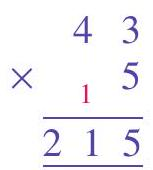
\includegraphics[max width=\textwidth]{2024_05_02_e8cf8b2d35d1e6495e29g-21}
\end{center}

\section*{Example 15}
Multiply 27 by 8 , using the short multiplication algorithm.

\section*{Solution}
27

\(\times \frac{58}{216}\)

\section*{Multiplication by more than one digit (the long multiplication algorithm)}
Consider \(378 \times 37\). The distributive law gives:

\[
\begin{aligned}
378 \times(30+7) & =378 \times 30+378 \times 7 \\
& =11340+2646 \\
& =13986
\end{aligned}
\]

An efficient setting out for this is as follows.

\begin{center}
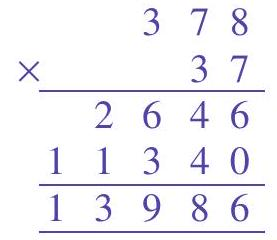
\includegraphics[max width=\textwidth]{2024_05_02_e8cf8b2d35d1e6495e29g-21(1)}
\end{center}

Multiplication by three digits is carried out in a similar way.

\begin{center}
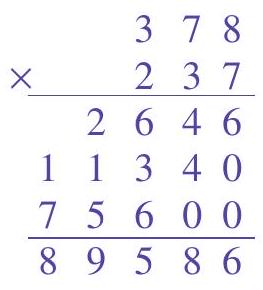
\includegraphics[max width=\textwidth]{2024_05_02_e8cf8b2d35d1e6495e29g-22(1)}
\end{center}

(Multiply by 7.)

(Multiply by 30. That is why the 0 is here.)

(Multiply by 200. That is why the 00 is here.)

To make the examples easy to read, we have left out all of the carry digits.

\section*{Example 16}
a Multiply 389 by 46.\\
b Multiply 667 by 667 .

\section*{Solution}
a

\begin{center}
\begin{tabular}{r}
389 \\
\(\times \quad 46\) \\
\hline
2334 \\
12560 \\
\hline
15994 \\
\hline
\end{tabular}
\end{center}

b

\begin{center}
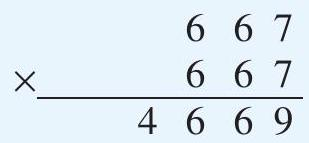
\includegraphics[max width=\textwidth]{2024_05_02_e8cf8b2d35d1e6495e29g-22}
\end{center}

\(\begin{array}{llllll}4 & 0 & 0 & 2 & 0\end{array}\)

\begin{center}
\begin{tabular}{llllll}
4 & 0 & 0 & 2 & 0 & 0 \\
\hline
4 & 4 & 4 & 8 & 8 & 9 \\
\hline
\end{tabular}
\end{center}

\section*{Exercise \(1 \mathrm{H}\)}
1 Carry out each calculation, using the short multiplication method.\\
a \(53 \times 4\)\\
b \(19 \times 8\)\\
c \(64 \times 7\)\\
d \(85 \times 4\)\\
e \(513 \times 4\)\\
f \(819 \times 8\)\\
g \(235 \times 7\)\\
h \(2006 \times 7\)\\
i \(6543 \times 7\)\\
j \(8159 \times 4\)\\
k \(91370 \times 9\)\\
l \(43987 \times 6\)

2 Carry out each calculation, using the long multiplication method.\\
a \(453 \times 24\)\\
b \(179 \times 86\)\\
c \(614 \times 47\)\\
d \(895 \times 45\)\\
e \(135 \times 27\)\\
f \(506 \times 68\)\\
g \(235 \times 34\)\\
h \(5646 \times 73\)\\
i \(91270 \times 39\)\\
j \(762 \times 549\)\\
k \(936 \times 564\)\\
l \(91370 \times 109\)

3 Calculate each of the following using either short or long multiplication.

a Each student in a class is given 9 coloured pencils by the teacher. How many pencils does the teacher need to supply 26 students?

b A packaging machine in a factory packs 893 boxes per hour. How many boxes are packed in a 12 -hour day?

c A brick wall has 43 rows of 723 bricks. How many bricks are in the wall?

d A publishing company packages books in boxes of 125 . How many books are there in 298 boxes?

4 A hall has 86 rows of 34 seats. How many seats are there in the hall?

5 A machine makes 257 doughnuts in an hour. How many doughnuts can it make in 13 hours?

6 Copy and complete the following by finding a digit for each \(\star\).\\
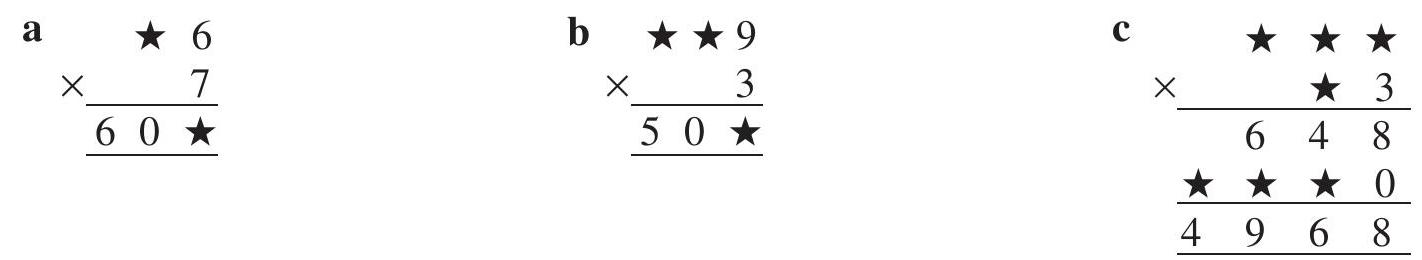
\includegraphics[max width=\textwidth, center]{2024_05_02_e8cf8b2d35d1e6495e29g-23}

7 A particular brand of lollies comes in packets of 26 . A carton contains 34 packets.

a How many lollies are there in one carton?

b How many lollies are there in 30 cartons?

8 A trolley at an airport is loaded with 15 cases, each with the maximum allowable weight of 20 kilograms. The trolley weighs 115 kilograms. What is the maximum possible weight of the trolley and the cases?

9 If 25 people each own 7 pairs of shoes, and 32 people each own 8 pairs of shoes, then how many shoes do the 57 people own in total?

10 Calculate your age in:\\
a months\\
b weeks\\
c days\\
d hours\\
e seconds

\section*{Division}
\section*{Division without remainder}
Division is an operation on two numbers that tells how many equal groups a number can be divided into. It can also tell how many are in each equal group.

Division without remainder is the reverse of multiplication. This is shown in the following example.

\section*{Example 17}
Fill in each box to give the equivalent multiplication or division statement.\\
a \(60 \div 5=12\) is equivalent to \(60=12 \times \square\).\\
b \(24 \div \square=4\) is equivalent to \(24=6 \times 4\).

Solution

a \(60 \div 5=12\) is equivalent to \(60=12 \times 5\). b \(24 \div 6=4\) is equivalent to \(24=6 \times 4\).

Division without remainder can answer questions such as:

'How many equal groups of 5 objects can 15 objects be divided into?'

This is shown in the diagram below.

\begin{center}
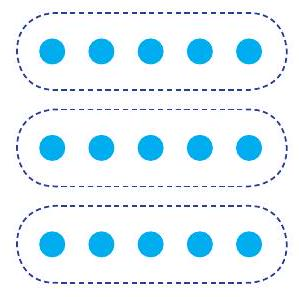
\includegraphics[max width=\textwidth]{2024_05_02_e8cf8b2d35d1e6495e29g-24(2)}
\end{center}

There are 3 such groups. The 15 objects are divided into 3 equal groups of 5 , so \(15 \div 5=3\).

The diagram also shows that \(15=5 \times 3\).

In addition, the diagram shows the answer to this question:

'If 15 objects are divided into three equal groups, how many objects are in each group?'

There are 5 objects in each group. The 15 objects are divided into three groups, each containing 5 objects.

\section*{Example 18}
There are 60 chocolates to be packed into boxes so that each box has 12 chocolates in it.

How many boxes are needed?

\section*{Solution}
As \(60=12 \times 5,5\) boxes are needed. That is, \(60 \div 12=5\).

\begin{center}
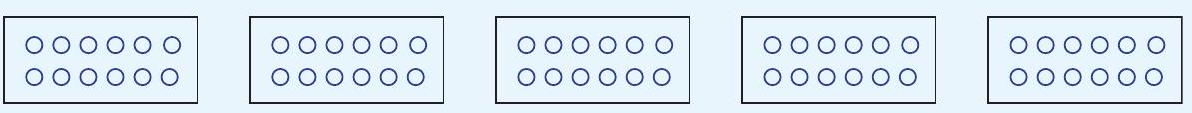
\includegraphics[max width=\textwidth]{2024_05_02_e8cf8b2d35d1e6495e29g-24(1)}
\end{center}

\section*{Example 19}
A box of 72 chocolates is to be divided equally between 9 people. How many chocolates does each person get?

\section*{Solution}
Each person gets \(72 \div 9=8\) chocolates.

\section*{Division with remainder}
If there are 28 marbles and you wish to form them into 3 equal groups, then the 28 marbles can be broken up into 3 groups of 9 marbles with 1 left over.

\begin{center}

\includegraphics[max width=\textwidth]{2024_05_02_e8cf8b2d35d1e6495e29g-24}
\end{center}

It is not possible to divide 28 into 3 equal groups, because 28 lies between \(3 \times 9=27\) and \(3 \times 10=30\). The best we can do is take 9 groups of 3 , with 1 left over. We can see this on a number line.

\begin{center}
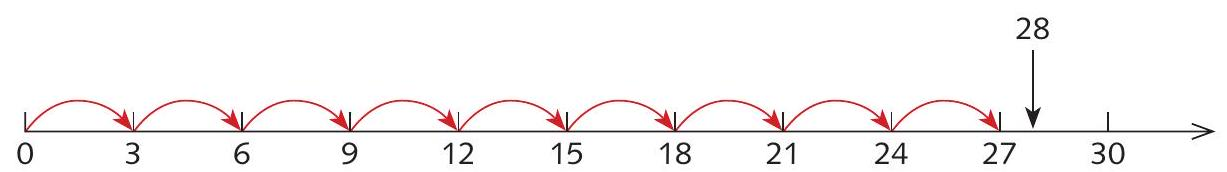
\includegraphics[max width=\textwidth]{2024_05_02_e8cf8b2d35d1e6495e29g-25}
\end{center}

This shows that \(28=3 \times 9+1\). We say ' \(28 \div 3\) equals 9 with remainder 1 '.

In this process, 28 is called the dividend, 3 is the divisor, 9 is the quotient and 1 is the remainder. The remainder must be less than the divisor.

\section*{Example 20}
Put the quotient in the first box and the remainder in the second box to make each statement true.\\
a \(26=\square \times 4+\square\)\\
b \(34=\square \times 3+\square\)

Solution\\
a \(26=6 \times 4+2\)\\
b \(34=[11 \times 3+1\)

\section*{Another notation for division}
Up to this point we have only used the sign \(\div\) for division. There is another way of writing division. For example:

\[
24 \div 6 \text { can also be written as } \frac{24}{6}
\]

Other examples using this notation are:

\[
\frac{0}{3}=0, \frac{72}{9}=8 \text { and } \frac{108}{12}=9
\]

For the time being, we will only use this notation for division without remainder. We will have more to say about this in Chapter 4 when we study fractions.

\section*{One and zero}
Any number divided by 1 gives the original number. For example:

\(3 \div 1=3\), and the equivalent multiplication statement is \(1 \times 3=3\)

Any number divided by itself gives 1 . For example:

\[
7 \div 7=1
\]

Dividing by 0 does not make sense. For example, if \(4 \div 0\) is a number, then that number multiplied by 0 is 4 . But multiplying any number by 0 gives 0 , so no such number exists.

However, 0 divided by any non-zero number is 0 . For example:

\[
0 \div 13=0 \text {, since } 13 \times 0=0
\]

\section*{Example 21}
Evaluate:\\
a \(\frac{25}{5}\)\\
b \(\frac{240}{3}\)

\section*{Solution}
a \(\frac{25}{5}=25 \div 5\)\\
b \(\frac{240}{3}=240 \div 3\)\\
\(=5\)\\
\(=80\)

\section*{The distributive law with division}
When dividing, it is sometimes useful to express the number you are dividing as a sum of two other numbers.

Here is a simple example, with a dot diagram to illustrate it. It uses the distributive law of division over addition.

\[
\begin{aligned}
16 \div 2 & =(10+6) \div 2 \\
& =10 \div 2+6 \div 2 \\
& =5+3 \\
& =8
\end{aligned}
\]

\begin{center}
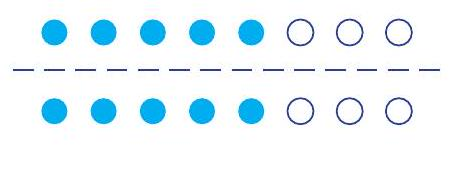
\includegraphics[max width=\textwidth]{2024_05_02_e8cf8b2d35d1e6495e29g-26}
\end{center}

Here is another example, this time involving subtraction. It uses the distributive law of division over subtraction.

\[
\begin{aligned}
196 \div 4 & =(200-4) \div 4 \\
& =200 \div 4-4 \div 4 \\
& =50-1 \\
& =49
\end{aligned}
\]

The distributive law for division over addition and subtraction makes it easier to carry out some divisions.

\section*{Example 22}
Use the distributive law to evaluate each of the following.\\
a \((100+55) \div 5\)\\
b \((200-15) \div 5\)\\
c \(540 \div 5\)

\section*{Solution}
a \((100+55) \div 5=100 \div 5+55 \div 5\)\\
\(=20+11\)\\
\(=31\)\\
b \((200-15) \div 5=200 \div 5-15 \div 5\)\\
\(=40-3\)\\
\(=37\)\\
c \(540 \div 5=(500+40) \div 5\)

\[
\begin{aligned}
& =500 \div 5+40 \div 5 \\
& =100+8 \\
& =108
\end{aligned}
\]

\section*{Properties of division}
\begin{itemize}
  \item The expression \(96 \div 8\) can mean: 'How many equal groups of 8 objects can be made from 96 objects?
  \item The expression \(96 \div 8\) can also mean: "If 96 objects are divided into 8 equal groups, how many objects are there in each group?'
  \item Division without remainder is the reverse operation of multiplication. For example, \(8 \times 12=96\) is equivalent to both \(96 \div 8=12\) and \(96 \div 12=8\).
  \item \(\ln 43=6 \times 7+1\) and \(43 \div 6=7\) remainder 1 , the number 43 is the dividend, 6 is the divisor, 7 is the quotient and 1 is the remainder.
  \item The distributive law works for division over addition. For example:
\end{itemize}

\[
\begin{aligned}
(700+25) \div 5 & =700 \div 5+25 \div 5 \\
& =140+5 \\
& =145
\end{aligned}
\]

\begin{itemize}
  \item The distributive law works for division over subtraction. For example:
\end{itemize}

\[
\begin{aligned}
(700-25) \div 5 & =700 \div 5-25 \div 5 \\
& =140-5 \\
& =135
\end{aligned}
\]

\section*{Exercise 11}
1 Fill in each box to give the equivalent multiplication or division statement.

a \(108 \div 9=12\) is equivalent to \(108=12 \times \square\).

b \(200 \div 10=20\) is equivalent to \(\square=10 \times 20\).

c \(72 \div \square=12\) is equivalent to \(72=12 \times \square\).

2 Work from left to right to calculate the following.\\
a \(24 \times 3 \div 3\)\\
b \(10 \times 2 \div 2\)\\
c \(36 \div 4 \times 4\)\\
d \(56 \div 8 \times 8\)\\
e \(18 \div 3 \times 3\)\\
f \(24 \div 12 \times 12\)

3 There are 28 chocolates to be divided equally among 4 people. How many chocolates does each person get?

4 There are 84 people at a club meeting. The organiser wishes to form 7 equal groups. How many people will there be in each group?

5 Fill in the boxes to make each statement true, with the smallest possible remainder.\\
a \(17=\square \times 3+\square\)\\
b \(37=\square \times 5+\square\)\\
c \(13=\square \times 2+\square\)\\
d \(87=\square \times 8+\square\)\\
e \(41=\square \times 5+\square\)\\
f \(148=\square \times 12+\square\)

6 Draw a dot diagram to show \(30 \div 8=3\) with remainder 6 or, equivalently, \(30=8 \times 3+6\).

7 Draw a dot diagram to show \(20 \div 6=3\) with remainder 2 or, equivalently, \(20=6 \times 3+2\).

8 Illustrate each expression on a number line.\\
a \(7 \div 2\)\\
b \(13 \div 3\)

9 Evaluate:\\
a \(\frac{20}{10}\)\\
b \(\frac{30}{6}\)\\
c \(\frac{42}{7}\)\\
d \(\frac{144}{12}\)\\
e \(\frac{36}{4}\)\\
f \(\frac{120}{3}\)

10 Perform each calculation by using the method indicated.

a \(448 \div 32\) (divide by 2 five times)

b \(640 \div 80\) (divide by 10 and then by 8 )

c \(805 \div 35\) (divide by 7 and then by 5 )

11 Evaluate each expression by using the distributive law.\\
a \((600+35) \div 5\)\\
b \((300-25) \div 5\)\\
c \(390 \div 5\)\\
d \((600+27) \div 3\)\\
e \((300-24) \div 3\)\\
f \(390 \div 3\)

\section*{The short division algorithm}
Consider 64 divided by 4 and 91 divided by 7 :

\[
\begin{aligned}
64 \div 4 & =(40 \div 4)+(24 \div 4) \\
& =10+6 \\
& =16
\end{aligned}
\]

\[
\begin{aligned}
91 \div 7 & =(70 \div 7)+(21 \div 7) \\
& =10+3 \\
& =13
\end{aligned}
\]

We can set this out as follows:\\
\(4 \longdiv { 6 ^ { 2 } 4 }\)\\
\(7 \longdiv { 9 ^ { 2 } 1 }\)

\section*{Example 23}
Find \(763 \div 4\).

\section*{Solution}
\(4) \frac{190}{7^{3} 63}\) remainder 3

\(763 \div 4=190\) remainder 3

In this example, 4 is first divided into 700 to give 100 with 300 remainder. We write 1 in the hundreds column to show this.

The remaining 300 is added to the 60 , then 4 is divided into 360 to give 90 exactly. We write 9 in the tens column.

Finally, 4 is divided into 3 to give 0 and 3 remainder. We write 0 in the ones column and a remainder of 3 at the end.

\section*{Example 24}
Find \(473 \div 4\).

\section*{Solution}
\(\frac{118}{4 \longdiv { 4 7 3 } \text { remainder } 1}\)

\(473 \div 4=118\) remainder 1

\section*{Example 25}
If \(\$ 6755\) is to be divided equally among 5 people, how much will each person receive?

\section*{Solution}
\(\frac{1351}{5 \longdiv { 6 ^ { 1 } 7 ^ { 2 } 5 5 }}\)

Each person will receive \(\$ 1351\).

\section*{Exercise \(1 \mathrm{l}\)}
1 Use short division to calculate:\\
a \(556 \div 2\)\\
b \(869 \div 7\)\\
c \(4536 \div 8\)\\
d \(8624 \div 8\)\\
e \(1089 \div 9\)\\
f \(5472 \div 6\)\\
g \(1496 \div 11\)\\
h \(33552 \div 12\)\\
i \(39240 \div 9\)

2 Work out each of the following, using short division.\\
a \(524 \div 4\)\\
b \(1095 \div 3\)\\
c \(498 \div 6\)\\
d \(431 \div 8\)\\
e \(740 \div 11\)\\
f \(9756 \div 12\)\\
g \(67543 \div 6\)\\
h \(19005 \div 7\)

3 If \(\$ 4250\) is to be divided equally among 5 people, how much will each person receive?

4 There are 542 tennis balls to be packed into boxes of 12 . How many boxes will be filled and how many tennis balls will be left over?

5 A biscuit company packages its biscuits into tins of 96 . The biscuits are arranged in rectangular arrays. How many rows with how many biscuits in each could there be? (Give four different answers.)

6 If 231 children from a school are to be transported on 7 buses, how many children will there be on each bus, if the number of children on each bus is the same?

7 There are 11 buses available to transport 407 people on an outing. How many people will there be on each bus, if the passengers are to be distributed equally?

8 A library of 3458 books is to be divided equally among 7 organisations. How many books will each organisation receive?

9 Eggs are sold in cartons of 12. If there are 345 eggs to be packaged, how many full cartons will there be and how many eggs will be left over?

10 Cans of lemonade are to be packaged together in groups of 6 . The factory has 4567 cans to be packaged. How many packages of 6 cans are there and how many are left over?

112552 people arrive at a film studio for a tour. The film studio decides that there should be exactly 8 people in a tour group.

a How many tour groups are there?

b How many people are left waiting to form the next group of 8 ?

\begin{center}

\includegraphics[max width=\textwidth]{2024_05_02_e8cf8b2d35d1e6495e29g-30(1)}
\end{center}

The long division algorithm is the short division algorithm with the subtractions set out. The long division algorithm is an efficient and clear way to set out division, particularly with larger divisions.

\begin{center}
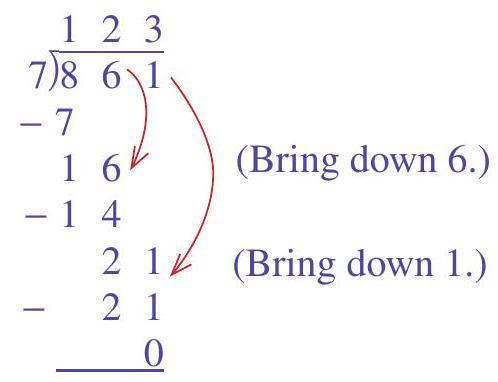
\includegraphics[max width=\textwidth]{2024_05_02_e8cf8b2d35d1e6495e29g-30}
\end{center}

The steps correspond to \(861-700=161\),

\[
\text { then } 161-140=21 \text {, } \quad
\]

and finally \(21-21=0\).

The answer, 123, is recorded on the top line.

Long division by larger numbers is more difficult because we do not know the multiples of large numbers in our heads. One of many possible methods is illustrated below. A table of the 9 multiples of the divisor is written on the right and then the appropriate multiple can easily be found.

\section*{Example 26}
Find \(8618 \div 27\), using the long division algorithm.

\section*{Solution}
\begin{center}
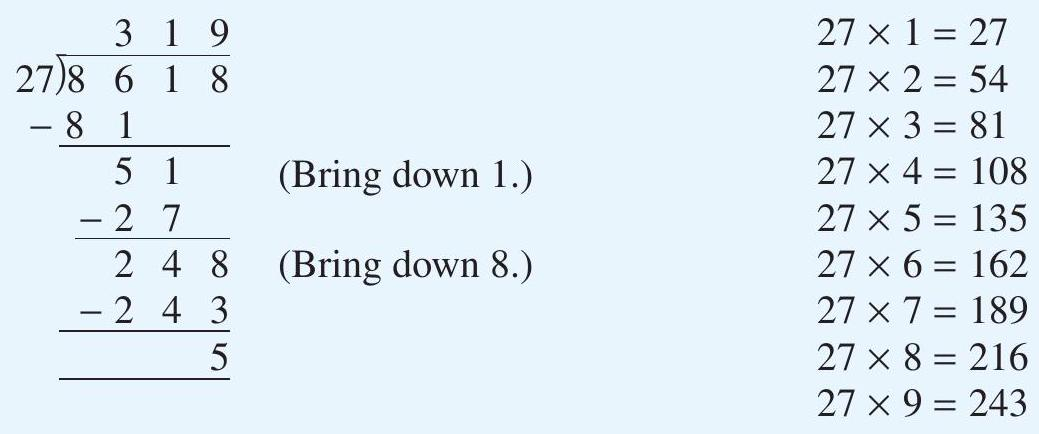
\includegraphics[max width=\textwidth]{2024_05_02_e8cf8b2d35d1e6495e29g-31}
\end{center}

\(8618 \div 27=319\) remainder 5

Note: Once the table is written down, the only arithmetic to be done is subtraction.

\section*{Exercise \(1 \mathrm{~K}\)}
1 Use the long division algorithm to calculate:\\
a \(728 \div 13\)\\
b \(1050 \div 14\)\\
c \(1344 \div 16\)\\
d \(4047 \div 19\)

2 Use the long division algorithm to calculate:\\
a \(2982 \div 71\)\\
b \(5244 \div 57\)\\
c \(3268 \div 43\)\\
d \(1743 \div 102\)

3 If \(\$ 4260\) is divided equally among 15 people, how much will each person receive?

4 If \(\$ 11572\) is divided equally among 22 people, how much will each person receive?

5 A piece of string that is \(1170 \mathrm{~cm}\) long is to be cut into 26 equal lengths. How long is each piece?

6 There are 5420 golf balls to be packed into boxes of 25 . How many boxes will be filled and how many golf balls will be left over?

7 If 1598 school children are to be transported on 34 buses, how many children will there be on each bus, if each bus contains the same number of children?

8 There are 27 buses available to transport 1107 fans to a football match. How many people will there be on each bus, if each bus contains the same number of people?

9 A computer program runs for 7568 seconds. Convert this to hours, minutes and seconds.

\section*{Order of operations}
There are important conventions for the order in which we carry out the arithmetic operations.

\section*{Order of operations}
\begin{itemize}
  \item Evaluate expressions inside brackets first.
  \item In the absence of brackets, carry out the operations in the following order:
  \item powers
  \item multiplication and division from left to right
  \item addition and subtraction from left to right.
\end{itemize}

\section*{Example 27}
a \(3 \times(5-1)\)\\
b \(7 \times 10^{2}\)\\
c \(4 \times 10 \div 2\)\\
d \(6+3 \times 4\)\\
e \(4+6-5+11\)\\
f \(7+84 \div 7\)

\section*{Solution}
a \(3 \times(5-1)=3 \times 4\)

\(=12\)

b \(7 \times 10^{2}=7 \times 100\)

\(=700\)

c \(4 \times 10 \div 2=40 \div 2\)

\(=20\)

d \(6+3 \times 4=6+12\)

\(=18\)

e \(4+6-5+11=10-5+11\)

\[
=5+11
\]

\(=16\)

f \(7+84 \div 7=7+12\)

\(=19\) (brackets first)

(powers first)

(multiplications and divisions from left to right)

(multiplication before addition)

(addition and subtraction from left to right)

(division before addition)

\section*{Exercise 1L}
1 Evaluate:\\
a \(6+7+11+8\)\\
b \(6+7+8-9\)\\
c \(4-3+6-2\)\\
d \(12-4-3+2\)\\
e \(7-1-3+6\)\\
f \(26-14-4+12\)\\
g \(56-28-20+2\)\\
h \(30+50-20-60\)\\
i \(32+8-40\)

2 Evaluate:\\
a \(34+5 \times 3\)\\
b \(60-4 \times 10\)\\
c \(52+45 \div 9\)\\
d \(45-45 \div 9\)\\
e \(66+23 \times 2\)\\
f \(24-144 \div 12\)

3 Evaluate:\\
a \(4 \div 10^{3}\)\\
b \(5+7-4+13\)\\
c \(5 \times 6 \div 3+7\)\\
d \((11-7) \times(12-5)\)\\
e \(4+28 \div 4\)\\
f \(64 \div 8+42 \div 7\)\\
g \(7+11 \times(5+7)\)\\
h \((14+11) \div 5\)\\
i \(10^{4} \times(2+11)\)

j \((24+56) \div(7+3)\)

4 Evaluate:\\
a \((4-3) \times 5\)\\
b \(24-15 \div 3\)\\
c \(3 \times(5-3)-6\)\\
d \((32-16)+(54-12) \div 6\)\\
e \(25 \div 5 \times 5 \div 25\)\\
f \(4 \times 11 \div 2 \times(12+8)\)\\
g \((75-45) \times 3+(11+9) \times 5\)\\
h \((7-4)+9 \div 3\)\\
i \((11+7) \div 3+8 \times(11+19)\)\\
j \((11+7) \div 3+8 \times 11+19\)

5 Insert brackets in each expression to make the resulting statement true.\\
a \(3 \times 6+4=30\)\\
b \(3 \times 7-6 \div 3=1\)\\
c \(8 \times 7+30 \div 5=104\)\\
d \(7 \times 3 \times 2+8=210\)\\
e \(5-2 \times 1+23 \div 6=12\)\\
f \(6+7 \times 11+1=156\)

6 Evaluate:\\
a \((4-3) \times 10^{2}\)\\
b \((340-140)-10^{2}\)\\
c \(3 \times 5-(13-6)\)\\
d \(10^{3} \div 5 \times 5 \div 25\)\\
e \(4 \times 10^{2} \div 2 \times(13+7)\)

7 Perform these calculations.\\
a Divide 36 by 3 and then add 6 .\\
b Add 6 to 36 and then divide by 3 .\\
c Subtract 12 from 64 and then divide by 4 .\\
d Add 15 to 210 and then divide by 5 .

8 Crates of bananas have 60 bananas in each. A market store owner buys 12 crates and 23 loose bananas. How many bananas does he buy?

9 Taj has 568 chocolates to give out at a party. He first divides the chocolates into 8 equal parcels. He then takes 3 of these parcels of chocolates and gives them to his friend Jane. How many chocolates does Jane receive?

10 Large crates of soft drinks each contain 56 bottles. It is decided that these are too heavy, so 8 bottles are removed from each crate. How many bottles are there in 15 of the lighter crates?

11 David divides \(\$ 4250\) equally between 5 bank accounts. He then adds another \(\$ 32\) to each of these accounts. How much money has he put into each account?

\section*{Review exercise}
1 Calculate:\\
a \(226+601+478\)\\
b \(72 \div 3\)\\
c \(163-136\)\\
d \(20 \div(9-4)+6\)\\
e \(8 \times 321+6\)\\
f \(68-42+12 \times 2\)\\
g \(382-792 \div 3\)\\
h \(268 \times(3+7)\)\\
i \((96 \div 3)+(258 \div 3)\)

2 The contents of a tin of chocolates weigh 6500 grams. The chocolates are divided into packets of 250 grams. How many packets are there?

3 There are 4000 apples to be divided into boxes so that each box holds 75 apples. How many boxes are required?

4 A club started the year with 125 members. During the year, 23 people left and 68 people joined. How many people belonged to the club at the end of the year?

5 If a bus can carry 45 passengers, how many buses are needed to transport 670 school students to a hockey game?

6 A supermarket takes delivery of 54 cartons of soft drink cans. Each carton contains 48 cans. How many cans are delivered?

7 On a school excursion, 17 buses each carry 42 students. How many students are transported?

8 A school day is 6 hours long. How many minutes are there in a school day?

9 Find the sum of eighty-six and fifty-four and then subtract sixty-eight.

10 The manager of the school canteen orders 1000 hot dogs for the week. On Monday 384 are sold and on Tuesday 239 are sold. How many hot dogs does the school have left for the rest of the week?

\section*{Challenge exercise}
1 Place the numbers 1,2,3, 4 and 5 in the circles of the following figure so that no two adjacent numbers (that is, numbers with a difference that is 1 ) are connected by a line.

\begin{center}
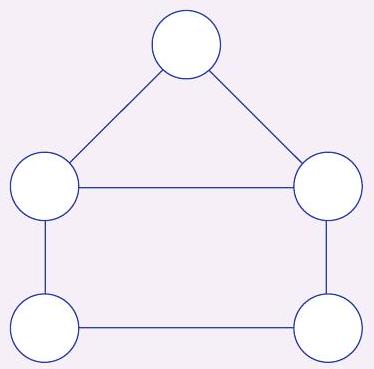
\includegraphics[max width=\textwidth]{2024_05_02_e8cf8b2d35d1e6495e29g-35(1)}
\end{center}

2 A palindromic number is a whole number that is unchanged when the order of the digits is reversed, for example, 131 and 34 543. The number 39793 is palindromic. Find the next 5 palindromic numbers.

3 Complete the following magic square, in which each row, column and diagonal must add up to the same sum.

\begin{center}
\begin{tabular}{|l|l|l|}
\hline
19 &  &  \\
\hline
 & 15 &  \\
\hline
22 &  & 11 \\
\hline
\end{tabular}
\end{center}

4 Place the numbers \(1,2,3,4,5\) and 6 in the circles of the following figure so that no two adjacent numbers are connected by a line.

\begin{center}
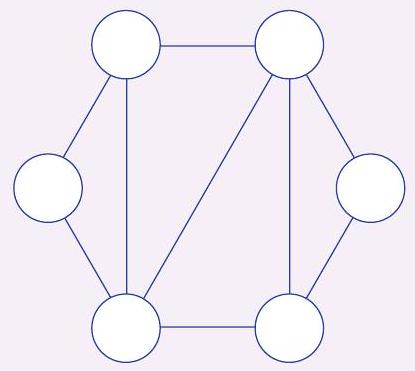
\includegraphics[max width=\textwidth]{2024_05_02_e8cf8b2d35d1e6495e29g-35}
\end{center}

5 Use five \(6 \mathrm{~s}\) and a selection of the symbols

\[
(,),+,-, \times \text { and } \div
\]

to write a statement with 66 as the result.

6 Using two straight lines, divide the clock face into three parts so that the sums of the numbers in each part are equal.

\begin{center}
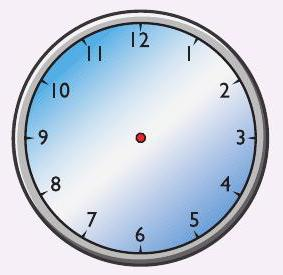
\includegraphics[max width=\textwidth]{2024_05_02_e8cf8b2d35d1e6495e29g-35(2)}
\end{center}

7 Place the numbers 1 to 9 in each of the circles in the following figure so that the sums of the numbers on each straight line are equal.

\begin{center}
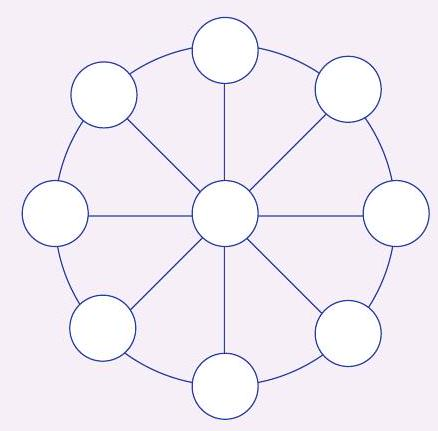
\includegraphics[max width=\textwidth]{2024_05_02_e8cf8b2d35d1e6495e29g-36}
\end{center}

8 Find a two-digit number that is twice the product of its digits.

9 Use all of the numbers \(1,2,3,4,5,6\) and 7 once and the symbols,,\(+- \times\) and \(\div\) to make a number sentence that results in 100 .

10 Place the numbers 1 to 9 in the circles to make each of the equations true.

\begin{center}
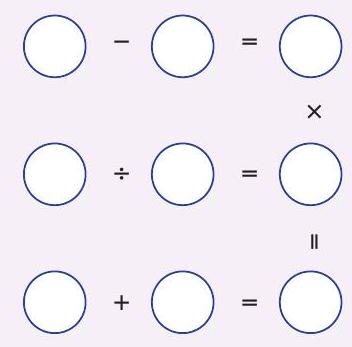
\includegraphics[max width=\textwidth]{2024_05_02_e8cf8b2d35d1e6495e29g-36(1)}
\end{center}

11 Place the numbers 1 to 9 in each of the circles in the following figure so that the sums of the numbers on each straight line are equal.

\begin{center}
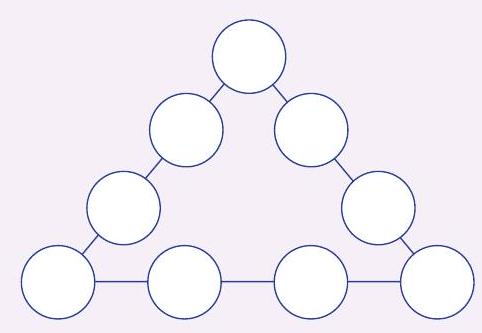
\includegraphics[max width=\textwidth]{2024_05_02_e8cf8b2d35d1e6495e29g-36(3)}
\end{center}

12 To protect his money from pickpockets, a merchant keeps his coins in several pouches so that he can pay any amount without revealing how much money he has, just by handing over the correct pouches. On the first day of trading he has six coins, so he places one coin in the first pouch, two coins in the second, and three coins in the third. This allows him to pay any value from one to six coins without having to open a pouch. The next day of trading he has 23 coins and five pouches. How should he distribute the coins to ensure that he can pay any amount from 1 to 23 coins?

13 Find the missing digits in the following multiplication.

\begin{center}
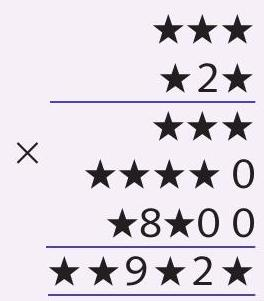
\includegraphics[max width=\textwidth]{2024_05_02_e8cf8b2d35d1e6495e29g-36(2)}
\end{center}

14 In each box below, place any number between 0 and 9 so that the number in the first box is the number of \(0 \mathrm{~s}\) in all the boxes, the number in the second box is the number of \(1 \mathrm{~s}\) in all the boxes, and so on.

\begin{center}
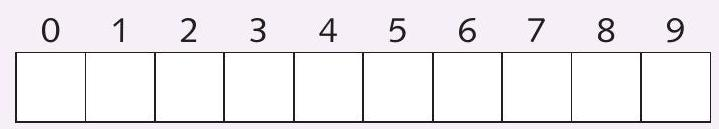
\includegraphics[max width=\textwidth]{2024_05_02_e8cf8b2d35d1e6495e29g-37}
\end{center}

15 Place the numbers 1 to 13 in the circles in the following figure so that the sums of the numbers on each straight line are equal.

\begin{center}
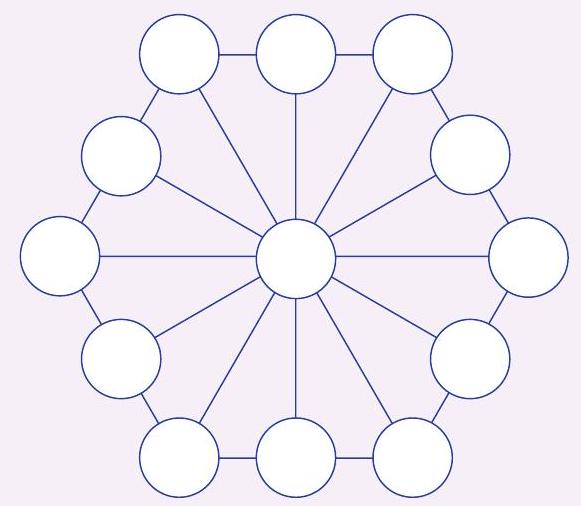
\includegraphics[max width=\textwidth]{2024_05_02_e8cf8b2d35d1e6495e29g-37(1)}
\end{center}

16 It is possible to choose four numbers such that any value between 1 and 40 can be made by taking one or more of these numbers and adding or subtracting them from each other. Find the four numbers, and show how the values from 1 to 40 can be made.

17 Using all the digits \(0,1,2,3,4,5,6,7,8\) and 9 , form two 5 -digit numbers so that their sum is:

a the greatest possible

b the smallest possible

18 A fast food store sells nuggets in boxes of 5 and 8 . You can buy 31 nuggets at a time since \(3 \times 5+2 \times 8=31\). What is the largest whole number of nuggets that cannot be purchased?

19 Find the sum of whole numbers from 1 to 100.


\end{document}